\documentclass[a4paper, 12pt]{article}

\usepackage[left=14mm, top=23mm, text={183mm, 252mm}]{geometry}
\usepackage[utf8]{inputenc}
\usepackage[slovak]{babel}
\usepackage{hyperref}
\usepackage{graphicx}
\usepackage{listings}
\usepackage{longtable}
\usepackage{float}
\usepackage{url}
\usepackage{tabularx}
\begin{document}

\begin{titlepage}
	\begin{center}
		{\Huge 
        \textsc{Vysoké učení technické v~Brně}\\[0.5em]}
		{\huge 
        \textsc{Fakulta informačních technologií}}\\
		\vspace{\stretch{0.382}}
		{\LARGE 
        Typografie a publikování -- 2.\ projekt\\[0.6em]
		PCAP NetFlow v5 exportér }
        \vspace{\stretch{0.618}}
	\end{center}
	{\Large 2024 \hfill 
    Michal Balogh (xbalog06) }
\end{titlepage}

\tableofcontents

\newpage

\section{Uvedenie do problematiky}

\subsection{Zadanie}

Za úlohu som mal vytvoriť program \texttt{p2nprobe}, ktorý bude extrahovať informácie o tokoch z PCAP súboru. Tieto toky bude odosielať na kolektor vo formáte NetFlow v5.

Program prijíma rôzne argumenty, pomocou ktorých sa dá nastaviť, ako budú toky agregované a kam ich bude odosielať (viz sekcia~\ref{sec:navod_na_pouzitie}).

Program bude na vstupe čítať pakety z PCAP súboru zadaného ako argument programu a tie spracuje a agreguje do tokov. Toky potom pomocou protokolu UDP odošle na NetFlow v5 kolektor, kde sú tieto toky ďalej spracované a analyzované. Program \texttt{p2nprobe} je len exporter a je zameraný len na záznamy o tokoch TCP.

\subsection{Základné informácie}

NetFlow v5 protokol vyvinutý spoločnosťou Cisco a slúži na monitorovanie a analýzu sieťového toku dát. Slúži na zbieranie informácií o sieťovej prevádzke a následnú analýzu na účely monitorovania, optimalizácie a bezpečnosti siete.

Toky sú agregované podľa určitých kritérií, ako sú napríklad IP adresa odosielateľa a prijímateľa, porty, protokol a ďalšie. Podľa nich sú prichádzajúce pakety jedinečne identifikovateľné a priradené do tokov.

Tok môže byť ukončený rôznymi spôsobmi. V programe \texttt{p2nprobe} je tok ukončený dvoma spôsobmi:
\begin{itemize}
    \item po uplynutí aktívneho timeoutu,
    \item po uplynutí neaktívneho timeoutu.
\end{itemize}

\textbf{Aktívny timeout} je časový interval, po ktorom je tok ukončený, aj keď do neho stále prichádzajú pakety.

\textbf{Neaktívny timeout} je časový interval, po ktorom je tok ukončený, ak do neho neprichádzajú žiadne pakety po nejaký čas.

\textbf{Exportér} expirované toky uchováva v pamäti a po nazbieraní maximálneho počtu tokov v pamäti alebo prečítaní posledného paketu zo súboru ich odošle na kolektor. Odoslaný UDP datagram obsahuje hlavičku a záznamy, ktorých podľa špecifikácie od spoločnosti Cisco je v rozsahu 1--30.

\section{Návrh aplikácie}

Program je rozdelený do viacerých logických častí, ktoré vykonávajú určité úlohy:
\begin{itemize}
    \item Načítanie argumentov programu a ich spracovanie -- \texttt{ArgParser},
    \item Načítanie paketov zo súboru a extrahovanie podstatných informácií -- \texttt{PcapReader},
    \item Správa a agregácia tokov -- \texttt{FlowManager},
    \item Odosielanie tokov na kolektor -- \texttt{Exporter}.
\end{itemize}

Program najprv spracuje vstupné argumenty a skontroluje ich validitu pomocou modulu \texttt{ArgParser}. Následne modul \texttt{PcapReader} načíta pakety zo súboru zadaného pomocou argumentu. Každý paket je spracovaný a sú z neho extrahované informácie, ktoré sú potrebné na identifikáciu toku a informácie potrebné pre štatistiky. Tieto informácie sú poslané do modulu \texttt{FlowManager}, ktorý z nich vytvorí jedinečný kľúč, pomocou ktorého identifikuje tok. Ak nejaký tok s týmto kľúčom existuje, aktualizuje ho, inak vytvorí nový. Ak \texttt{FlowManager} vyhodnotí tok ako expirovaný pomocou informácií z paketu alebo informácií od modulu \texttt{PcapReader}, že prečítal posledný paket z PCAP súboru, je odoslaný na kolektor pomocou modulu \texttt{Exporter}.

\section{Popis implementácie}

Nižšie je zobrazený class diagram, ktorý zobrazuje, ako sú jednotlivé moduly programu \texttt{p2nprobe} implementované a ako spolu komunikujú.

\newpage
\subsection{Diagram}

\begin{figure}[H]
    \centering
    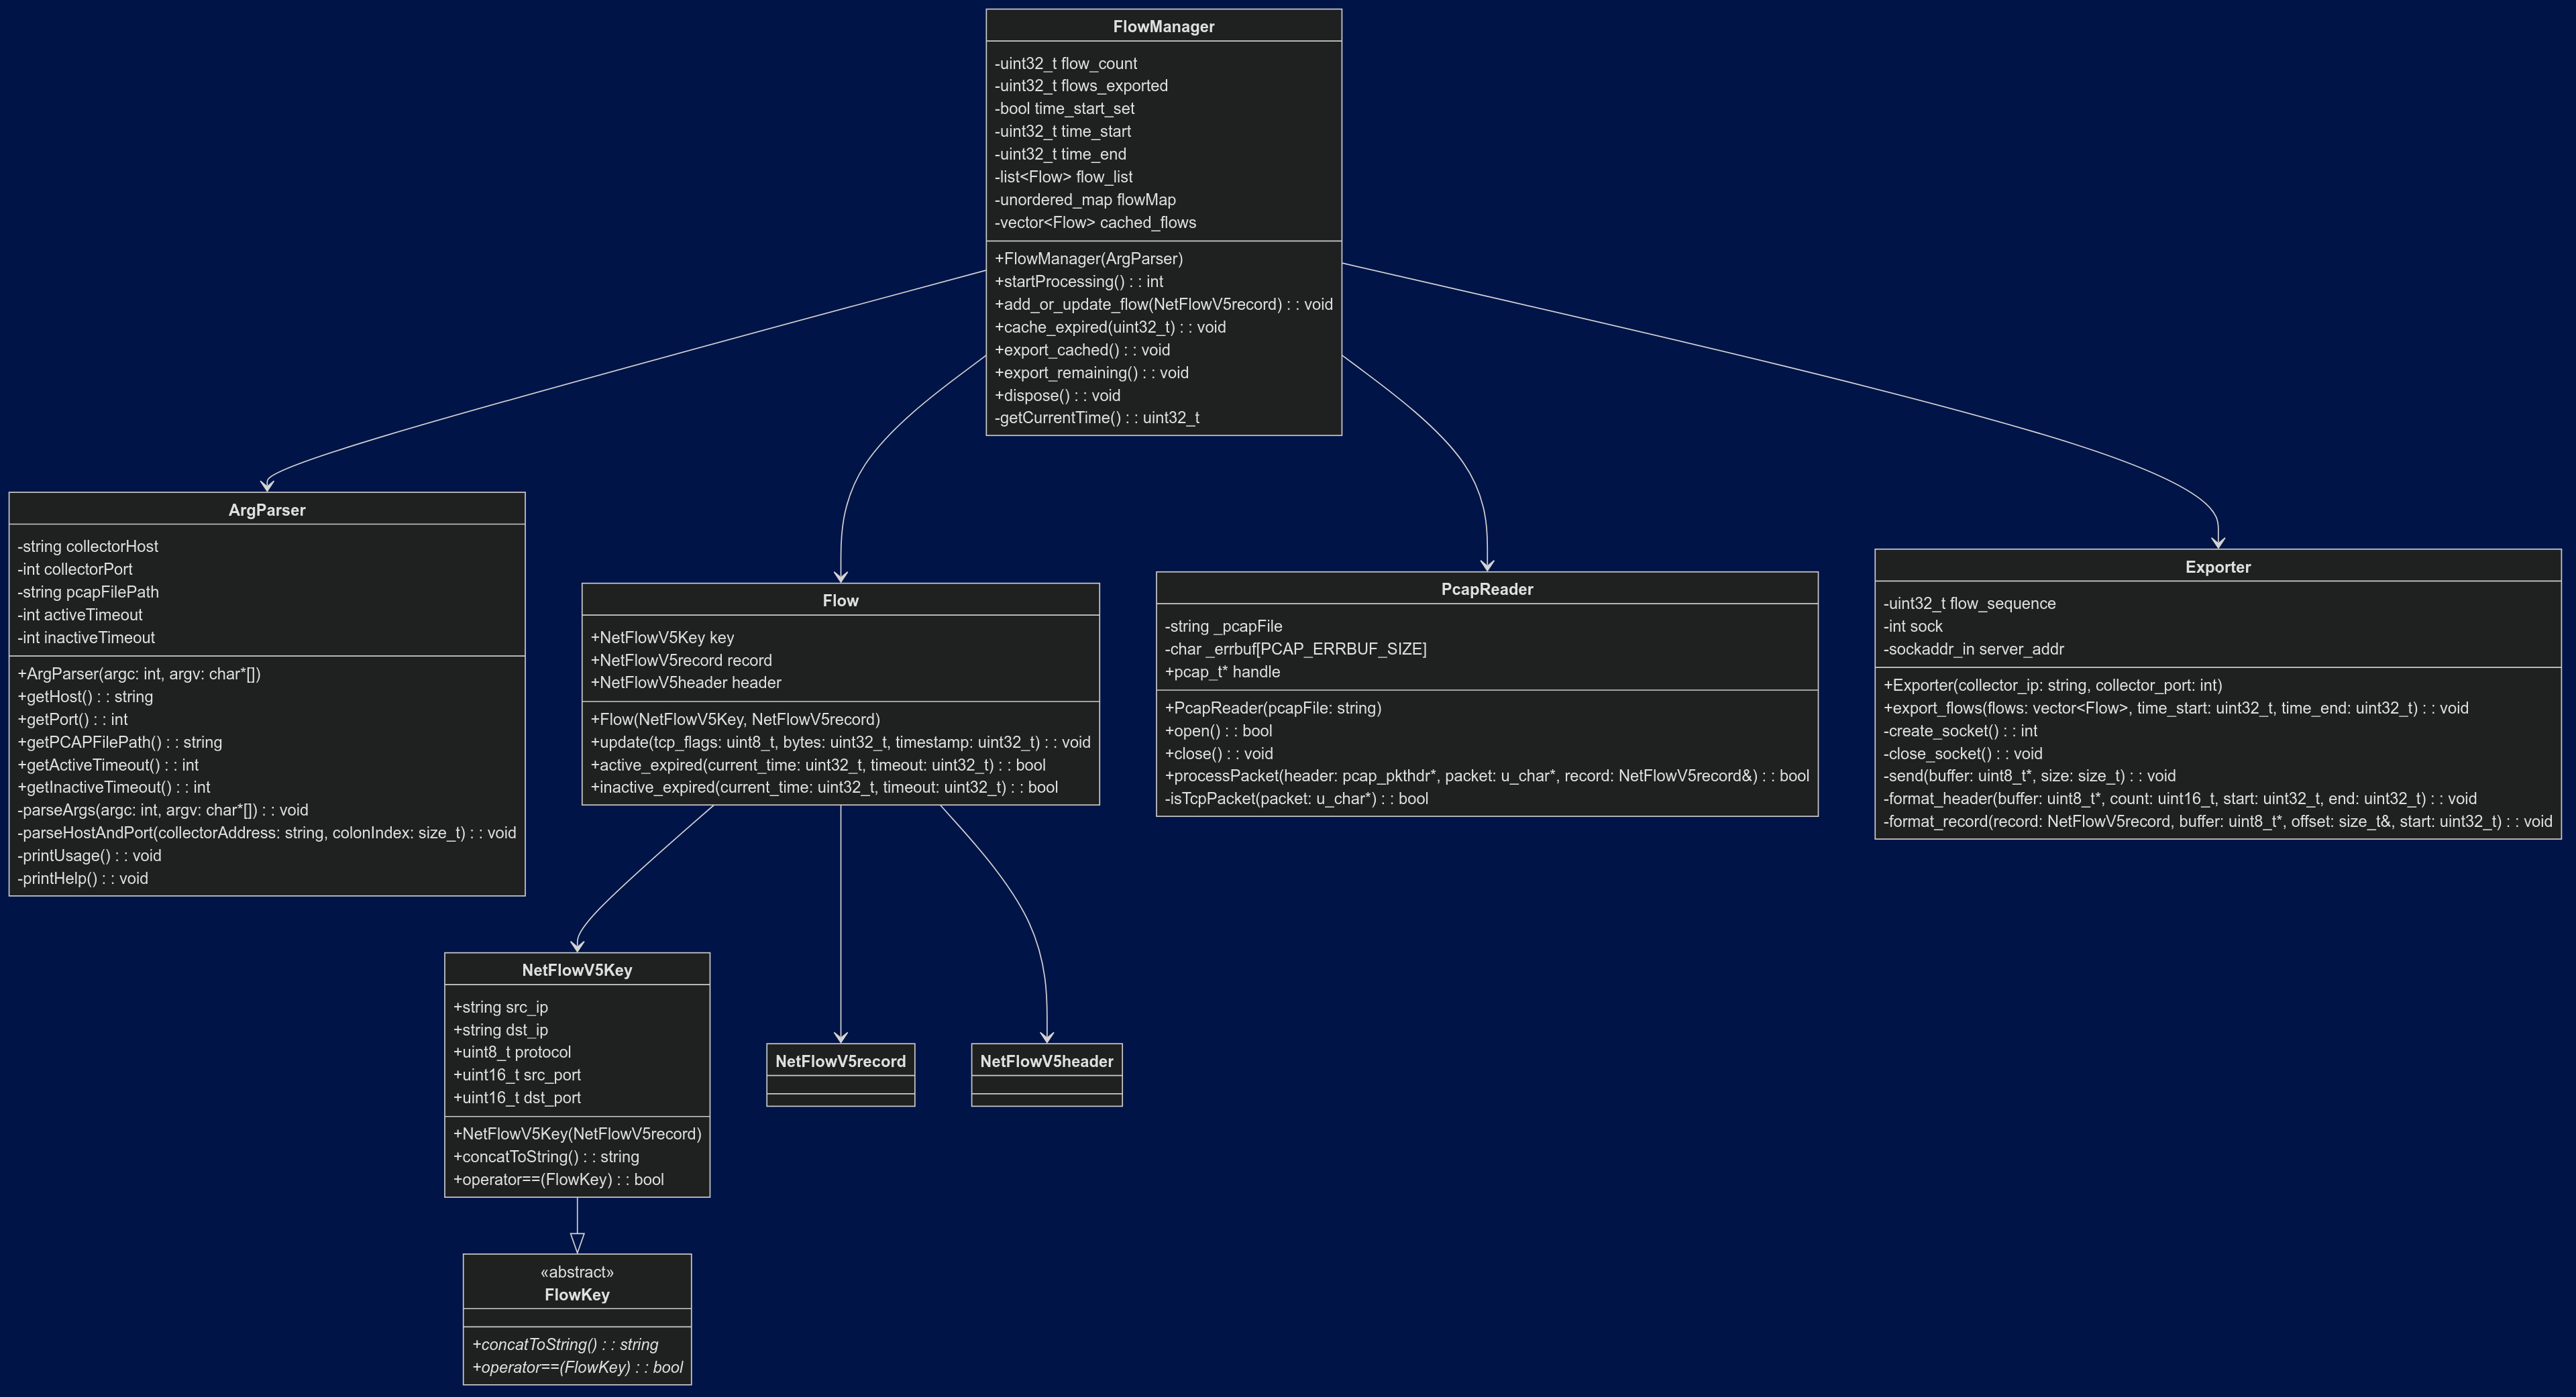
\includegraphics[width=1.2\textwidth, angle=90]{class_diagram.png}
    \caption{Class diagram}
\end{figure}
\newpage

\subsection{Implementácia}

Program \texttt{p2nprobe} je implementovaný v jazyku C++ verzia C++17 a využíva knižnicu \texttt{libpcap} na čítanie a spracovanie paketov.

\subsubsection{Použité knižnice}

\begin{itemize}
    \item \textbf{libpcap} -- čítanie PCAP súborov a extrahovanie informácií z paketov,
    \item \textbf{arpa/inet.h} -- konverzia IP adries a portov medzi sieťovým a hostiteľským formátom,
    \item \textbf{netinet/ip.h}, \textbf{netinet/tcp.h} -- parsovanie sieťových hlavičiek,
    \item \textbf{sys/socket.h} -- odosielanie NetFlow záznamov na kolektor,
    \item \textbf{unordered\_map}, \textbf{vector}, \textbf{string} -- ukladanie a správa tokov a záznamov,
    \item \textbf{ctime}, \textbf{chrono} -- práca s časovými značkami a meranie času,
    \item \textbf{iostream}, \textbf{sstream} -- formátovanie výstupu (správa help, rôzne chybové hlášky),
    \item \textbf{memory} -- smart pointre a správa pamäte.
\end{itemize}

\subsection{Konkrétne moduly}

\subsubsection{ArgParser}
Modul na načítanie vstupných argumentov programu, spracovanie a overenie, či sú argumenty validné. V prípade chyby alebo chýbajúcich povinných argumentov vypíše chybovú hlášku a ukážku, ako spustiť program. Argument -h vypíše ``help'' správu, ktorá informuje užívateľa o použití programu a jednotlivých argumentoch.

\subsubsection{ErrorCodes}
Definície rôznych chybových hlášok pre lepšie rozpoznávanie, aká chyba nastala.
Možné chybové kódy:
\begin{itemize}
    \item 0 - Bez chyby
    \item 1 - Vnútorná chyba, napríklad chyba alokácie pamäti
    \item 2 - Nesprávne argumenty
    \item 3 - Chyba pri otváraní súboru
    \item 4 - Chyba pri čítaní paketu
    \item 5 - Paket obsahuje nevalidné informácie
\end{itemize}

Implementuje aj funkciu ExitWith pre konzistentné ukončenie programu, na zjednodušenie správy chybových stavov.

\subsubsection{PcapReader}
Trieda na čítanie paketov zo súboru a ich spracovanie. Poskytuje rozhranie pre extrakciu TCP paketov a základných informácií z paketov a tie uloží do štruktúry NetFlowV5record. Konštruktor triedy PcapReader má jeden parameter - cestu k PCAP súboru, ktorý sa má čítať. Metóda \texttt{processPacket} načíta jeden paket a spracuje ho. Metóda \texttt{isTcpPacket} kontroluje, či je daný paket TCP paket - ostatné pakety sú ignorované.

\subsubsection{FlowManager}
Hlavná trieda zodpovedná za správu a agregáciu tokov. Rieši komunikáciu medzi jednotlivými triedami. Vytvára toky a kľúče pre ne podľa informácií z paketu. Pomocou týchto kľúčov potom vie identifikovať, či tok už existuje alebo nie. Ak tok existuje, pridá paket do toku pomocou metódy \texttt{add\_or\_update\_flow}. Ak tok neexistuje, vytvorí nový tok a pridá paket do neho. Na efektívne vyhľadávanie využíva kombinovanú dátovú štruktúru (hash mapa + linked list) pre efektívne vyhľadávanie a správu tokov. Hash mapa slúži na rýchle vyhľadanie tokov pomocou kľúča a linked list obsahuje odkazy do hashmapy, ale zároveň udržuje poradie, v akom sa toky vytvorili. Toky, ktoré expirovali neexportuje hneď, ale ``cachuje'' pomocou metódy \texttt{cache\_expired} a exportuje ich až keď je naplnený maximálny počet tokov v pamäti (30) alebo je prečítaný posledný paket zo súboru. Má dve metódy na exportovanie tokov na kolektor - \texttt{export\_cached} a \texttt{export\_remaining}. Prvá metóda exportuje všetky toky, ktoré sú uložené v cache keď sa naplní kapacita, druhá metóda exportuje všetky toky, keď sa načíta posledný paket ale zároveň cache ešte nie je plná.

\subsubsection{NetFlowV5Key}
Implementácia unikátneho kľúča pre identifikáciu tokov. Kombinuje 5 kľúčových atribútov: zdrojová/cieľová IP, porty a protokol pre jednoznačnú identifikáciu toku. Využíva preťaženie operátora \texttt{==} pre porovnávanie kľúčov a implementuje vytvorenie kľúča (jednoduchá konkatenácia všetkých atribútov kľúča) z údajov, ktoré sú mu dané pre použitie v hash mape.

\subsubsection{Exporter}
Modul pre formátovanie a export NetFlow záznamov na kolektor. Modul formátuje NetFlow záznamy (štruktúra NetFlowV5record) a NetFlow hlavičky (štruktúra NetFlowV5header) podľa špecifikácie NetFlow v5 a odosiela ich na kolektor špecifikovaný v programových argumentoch pomocou protokolu UDP. Okrem toho aj počíta počet odoslaných paketov, keďže tento údaj je potrebný v hlavičke NetFlow záznamu. Podporuje resolvovanie hostname na IP adresu pomocou funkcie \texttt{getaddrinfo} (knižnica \texttt{arpa/inet.h}).

\subsubsection{Flow}
Reprezentácia jednotlivého sieťového toku, ktorá zapuzdruje všetky potrebné informácie o toku a jeho štatistiky. Taktiež obsahuje metódy na pridanie paketu do toku a kontrolu, či je tok expirovaný buď pomocou aktívneho alebo neaktívneho timeoutu. Jeho konštruktor má 2 parametre - kľúč, podľa ktorého je daný flow identifikovateľný a prvý záznam z paketu, ktorý je pridaný do toku.

\newpage

\subsubsection{Štruktúra NetFlowV5header}
Štruktúra, ktorá reprezentuje hlavičku NetFlow záznamu. Obsahuje informácie uvedené v tabuľke nižšie alebo v dokumentácii od spoločnosti Cisco\cite{cisco}\cite{ibm}.

\begin{table}[h]
\centering
\begin{tabular}{|l|l|l|}
\hline
\textbf{Offset} & \textbf{Field} & \textbf{Popis} \\
\hline
0-1 & version & Číslo verzie formátu exportu NetFlow \\
2-3 & count & Počet tokov exportovaných v tomto pakete (1-30) \\
4-7 & SysUptime & Aktuálny čas v milisekundách od spustenia exporteru \\
8-11 & unix\_secs & Aktuálny počet sekúnd od 0000 UTC 1970 \\
12-15 & unix\_nsecs & Zvyškové nanosekundy od 0000 UTC 1970 \\
16-19 & flow\_sequence & Počítadlo sekvencie celkového počtu tokov \\
20 & engine\_type & Typ engine-u na prepínanie tokov \\
21 & engine\_id & Číslo slotu engine-u na prepínanie tokov \\
22-23 & sampling\_interval & Prvé dva bity obsahujú režim vzorkovania; zvyšných 14 bitov obsahuje hodnotu intervalu vzorkovania \\
\hline
\end{tabular}
\end{table}

\subsubsection{Štruktúra NetFlowV5record}
Štruktúra, ktorá reprezentuje záznam NetFlow v5. Obsahuje informácie uvedené v tabuľke nižšie alebo v dokumentácii od spoločnosti Cisco\cite{cisco}\cite{ibm}.

\begin{table}[h]
\centering
\begin{tabular}{|l|l|l|}
\hline
\textbf{Bajty} & \textbf{Obsah} & \textbf{Popis} \\
\hline
0-3 & srcaddr & Zdrojová IP adresa \\
4-7 & dstaddr & Cieľová IP adresa \\
8-11 & nexthop & IP adresa ďalšieho smerovača \\
12-13 & input & SNMP index vstupného rozhrania \\
14-15 & output & SNMP index výstupného rozhrania \\
16-19 & dPkts & Počet paketov v toku \\
20-23 & dOctets & Celkový počet bajtov vrstvy 3 \\
24-27 & First & SysUptime na začiatku toku \\
28-31 & Last & SysUptime v čase prijatia posledného paketu toku \\
32-33 & srcport & Zdrojový port TCP/UDP alebo ekvivalent \\
34-35 & dstport & Cieľový port TCP/UDP alebo ekvivalent \\
36 & pad1 & Nepoužité (nulové) bajty \\
37 & tcp\_flags & Kumulatívny OR TCP príznakov \\
38 & prot & Typ IP protokolu (napríklad TCP = 6; UDP = 17) \\
39 & tos & IP typ služby (ToS) \\
40-41 & src\_as & Číslo autonómneho systému zdroja \\
42-43 & dst\_as & Číslo autonómneho systému cieľa \\
44 & src\_mask & Bitová maska zdrojovej adresy \\
45 & dst\_mask & Bitová maska cieľovej adresy \\
46-47 & pad2 & Nepoužité (nulové) bajty \\
\hline
\end{tabular}
\end{table}


\section{Návod na použitie}
\label{sec:navod_na_pouzitie}

\subsection{Kompilácia programu}

Program je možné skompilovať pomocou \texttt{Makefile}. Pre kompiláciu programu je potrebné mať nainštalované knižnice \texttt{libpcap} a \texttt{g++} (verzia C++17). Preloženie programu je možné pomocou príkazu:
\begin{lstlisting}[language=bash]
make
\end{lstlisting}

\subsection{Spustenie programu}

Program je možné spustiť takto:
\begin{lstlisting}[language=bash]
./p2nprobe <host>:<port> <pcap_file_path> [-a <active_timeout> -i <inactive_timeout>]
\end{lstlisting}

Kde:

\begin{itemize}
    \item \texttt{<pcap\_file\_path>} -- cesta k PCAP súboru, ktorý sa má čítať,
    \item \texttt{<host>} -- IP adresa kolektora, kam sa majú odosielať toky,
    \item \texttt{<port>} -- port kolektora, kam sa majú odosielať toky,
    \item \texttt{-a <active\_timeout>} -- aktívny timeout, po ktorom je tok ukončený (defaultná hodnota 60 sekúnd),
    \item \texttt{-i <inactive\_timeout>} -- neaktívny timeout, po ktorom je tok ukončený (defaultná hodnota 60 sekúnd).
\end{itemize}

Poradie parametrov je ľubovoľné.

Ukážka spustenia programu:
\begin{lstlisting}[language=bash]
./p2nprobe localhost:9995 pcap_file.pcap -a 5 -i 30

./p2nprobe 127.0.0.1:9995 pcap_file.pcap
\end{lstlisting}

Keďže \texttt{p2nprobe} je len exporter, je potrebné mať spustený NetFlow kolektor, ktorý bude prijímať toky. Napríklad pomocou programu \texttt{nfcapd}:
\begin{lstlisting}[language=bash]
nfcapd -l . -p 9995
\end{lstlisting}

Následne je možné sledovať toky pomocou programu \texttt{nfdump}:
\begin{lstlisting}[language=bash]
nfdump -r nfcapd.202411052020
\end{lstlisting}


\newpage
\section{Popis testovania aplikácie}

Aplikáciu som testoval pomocou odporúčaného programu ako referenciu -- \texttt{softflowd}\cite{softflowd}. NetFlow toky som zachytával pomocou programu \texttt{nfcapd}.

\begin{lstlisting}[language=bash]
nfcapd -l . -p 9995        
\end{lstlisting}

V druhom termináli som potom spustil:

\begin{lstlisting}[language=bash]
sudo softflowd -r netflow_capture1.pcap -n localhost:9995
\end{lstlisting}

Bohužiaľ, aktívny a neaktívny timeout v \texttt{softflowd} nefungoval, takže som mohol testovať len predvolené hodnoty.

Následne som toky analyzoval a porovnával pomocou programu \texttt{nfdump}.

\begin{lstlisting}[language=bash]
nfdump -r nfcapd.202411052100
\end{lstlisting}

Takto som získal referenčný výstup. Tento postup som opakoval pre môj program \texttt{p2nprobe}.

Na porovnanie som si vytvoril Python skript, ktorý porovnáva výstupy od \texttt{nfdump} pre oba programy.

Keďže nebolo možné takto testovať aktívny a neaktívny timeout, tak som potom zachytával pomocou vlastného Python skriptu \texttt{test\_probe.py}, ktorý vie vypísať všetky údaje z NetFlow záznamov, ale aj porovnať s iným kolektorom, napríklad \texttt{softflowd}.

\section{Výsledky testov}

\newpage

\section{Bibliografia}
\begin{thebibliography}{99}

\bibitem{cplusplus}
CPlusPlus.com,
\emph{C++ Reference},
[Online]. Dostupné na: \url{https://cplusplus.com/reference/}
[Citované: \today]

\bibitem{w3schools}
W3Schools,
\emph{C++ OOP},
[Online]. Dostupné na: \url{https://www.w3schools.com/cpp/cpp_oop.asp}
[Citované: \today]

\bibitem{ibm}
IBM Documentation,
\emph{NetFlow V5 Formats},
[Online]. Dostupné na: \url{https://www.ibm.com/docs/en/npi/1.3.0?topic=versions-netflow-v5-formats}
[Citované: \today]

\bibitem{cisco}
Cisco Systems,
\emph{NetFlow Collection Engine User Guide},
[Online]. Dostupné na: \url{https://www.cisco.com/c/en/us/td/docs/net_mgmt/netflow_collection_engine/3-6/user/guide/format.html}
[Citované: \today]

\bibitem{tcpdump}
Tcpdump/Libpcap,
\emph{PCAP Documentation},
[Online]. Dostupné na: \url{https://www.tcpdump.org/pcap.html}
[Citované: \today]

\bibitem{pcapreader}
Voldemur,
\emph{PCAP Reader Implementation},
GitHub Gist,
[Online]. Dostupné na: \url{https://gist.github.com/voldemur/261b5bc42688b9cf425fbaedc2d5fcbe#file-pcap_reader-cpp}
[Citované: \today]

\bibitem{inetntop}
Linux manual pages,
\emph{inet\_ntop(3) - Linux manual page},
[Online]. Dostupné na: \url{https://man7.org/linux/man-pages/man3/inet_ntop.3.html}
[Citované: \today]

\bibitem{getaddrinfo}
Linux manual pages,
\emph{getaddrinfo(3) - Linux manual page},
[Online]. Dostupné na: \url{https://man7.org/linux/man-pages/man3/getaddrinfo.3.html}
[Citované: \today]

\bibitem{scaler}
Scaler Topics,
\emph{Virtual Base Class in C++},
[Online]. Dostupné na: \url{https://www.scaler.com/topics/virtual-base-class-in-cpp/}
[Citované: \today]

\bibitem{geeksforgeeks}
GeeksforGeeks,
\emph{Copy Constructor in C++},
[Online]. Dostupné na: \url{https://www.geeksforgeeks.org/copy-constructor-in-cpp/}
[Citované: \today]

\bibitem{educative}
Educative.io,
\emph{How to implement UDP sockets in C},
[Online]. Dostupné na: \url{https://www.educative.io/answers/how-to-implement-udp-sockets-in-c}
[Citované: \today]

\bibitem{softflowd}
Irino,
\emph{softflowd},
GitHub repository,
[Online]. Dostupné na: \url{https://github.com/irino/softflowd/}
[Citované: \today]

\end{thebibliography}

\end{document}